\thispagestyle{duongvaotoanhocnone}
\pagestyle{duongvaotoanhoc}
\everymath{\color{duongvaotoanhoc}}
\graphicspath{{../duongvaotoanhoc/pic/}}
\blfootnote{$^1$\color{duongvaotoanhoc}Nguồn: \url{https://plus.maths.org}}
\begingroup
\AddToShipoutPicture*{\put(0,616){\includegraphics[width=19.3cm]{../bannerduongvao}}}
\AddToShipoutPicture*{\put(92,503){\includegraphics[scale=1]{../tieude.pdf}}}
\centering
\endgroup

\vspace*{200pt}


\begin{multicols}{2}	
	Huy chương Chern năm nay đã được trao cho Barry Mazur, giáo sư toán của Đại học Harvard. Huy chương Chern được trao bốn năm một lần tại Đại hội Toán học Thế giới ``cho một cá nhân có những thành tích đảm bảo mức ghi nhận cao nhất dành cho những thành tựu đặc biệt xuất sắc trong lĩnh vực toán học".
	\vskip 0.05cm
	Mazur đã nhận được huy chương vì ``những khám phá sâu sắc trong tô pô, hình học số học và lý thuyết số, cũng như năng lực dẫn dắt và sự ân cần của ông trong việc đào tạo thế hệ những nhà toán học tiếp theo".
	\vskip 0.05cm
	Chúng tôi may mắn được nói chuyện với Mazur trong thời gian chuẩn bị cho Đại hội Toán học thế giới năm nay, được tổ chức với hình thức hỗn hợp giữa trực tiếp và trực tuyến, trong đó phần trực tiếp diễn ra tại Helsinki, Phần Lan. Ông kể cho chúng tôi nghe một câu chuyện đáng kinh ngạc về những thay đổi về chủ đề nghiên cứu, những hướng đi mới và một cái nhìn rất riêng về toán học.
	\vskip 0.05cm
	\textbf{\color{duongvaotoanhoc}Từ đài phát thanh đến hình học của miếng cao su}
	\vskip 0.05cm
	Mazur đến với toán học từ sự yêu thích đối với truyền thanh. ``Vật lý của đài phát thanh, với những điều bí ẩn và kỳ diệu của nó, đã khiến tôi bị cuốn hút khi tôi $12$ tuổi," ông nói. Ở trường trung học, ông trở thành một kỹ thuật viên phát thanh nghiệp dư, gửi tin nhắn bằng mã Morse tới các kỹ thuật viên khác ở khắp nơi trên thế giới.
	\begin{figure}[H]
		\centering
		\vspace*{-5pt}
		\captionsetup{labelformat= empty, justification=centering}
		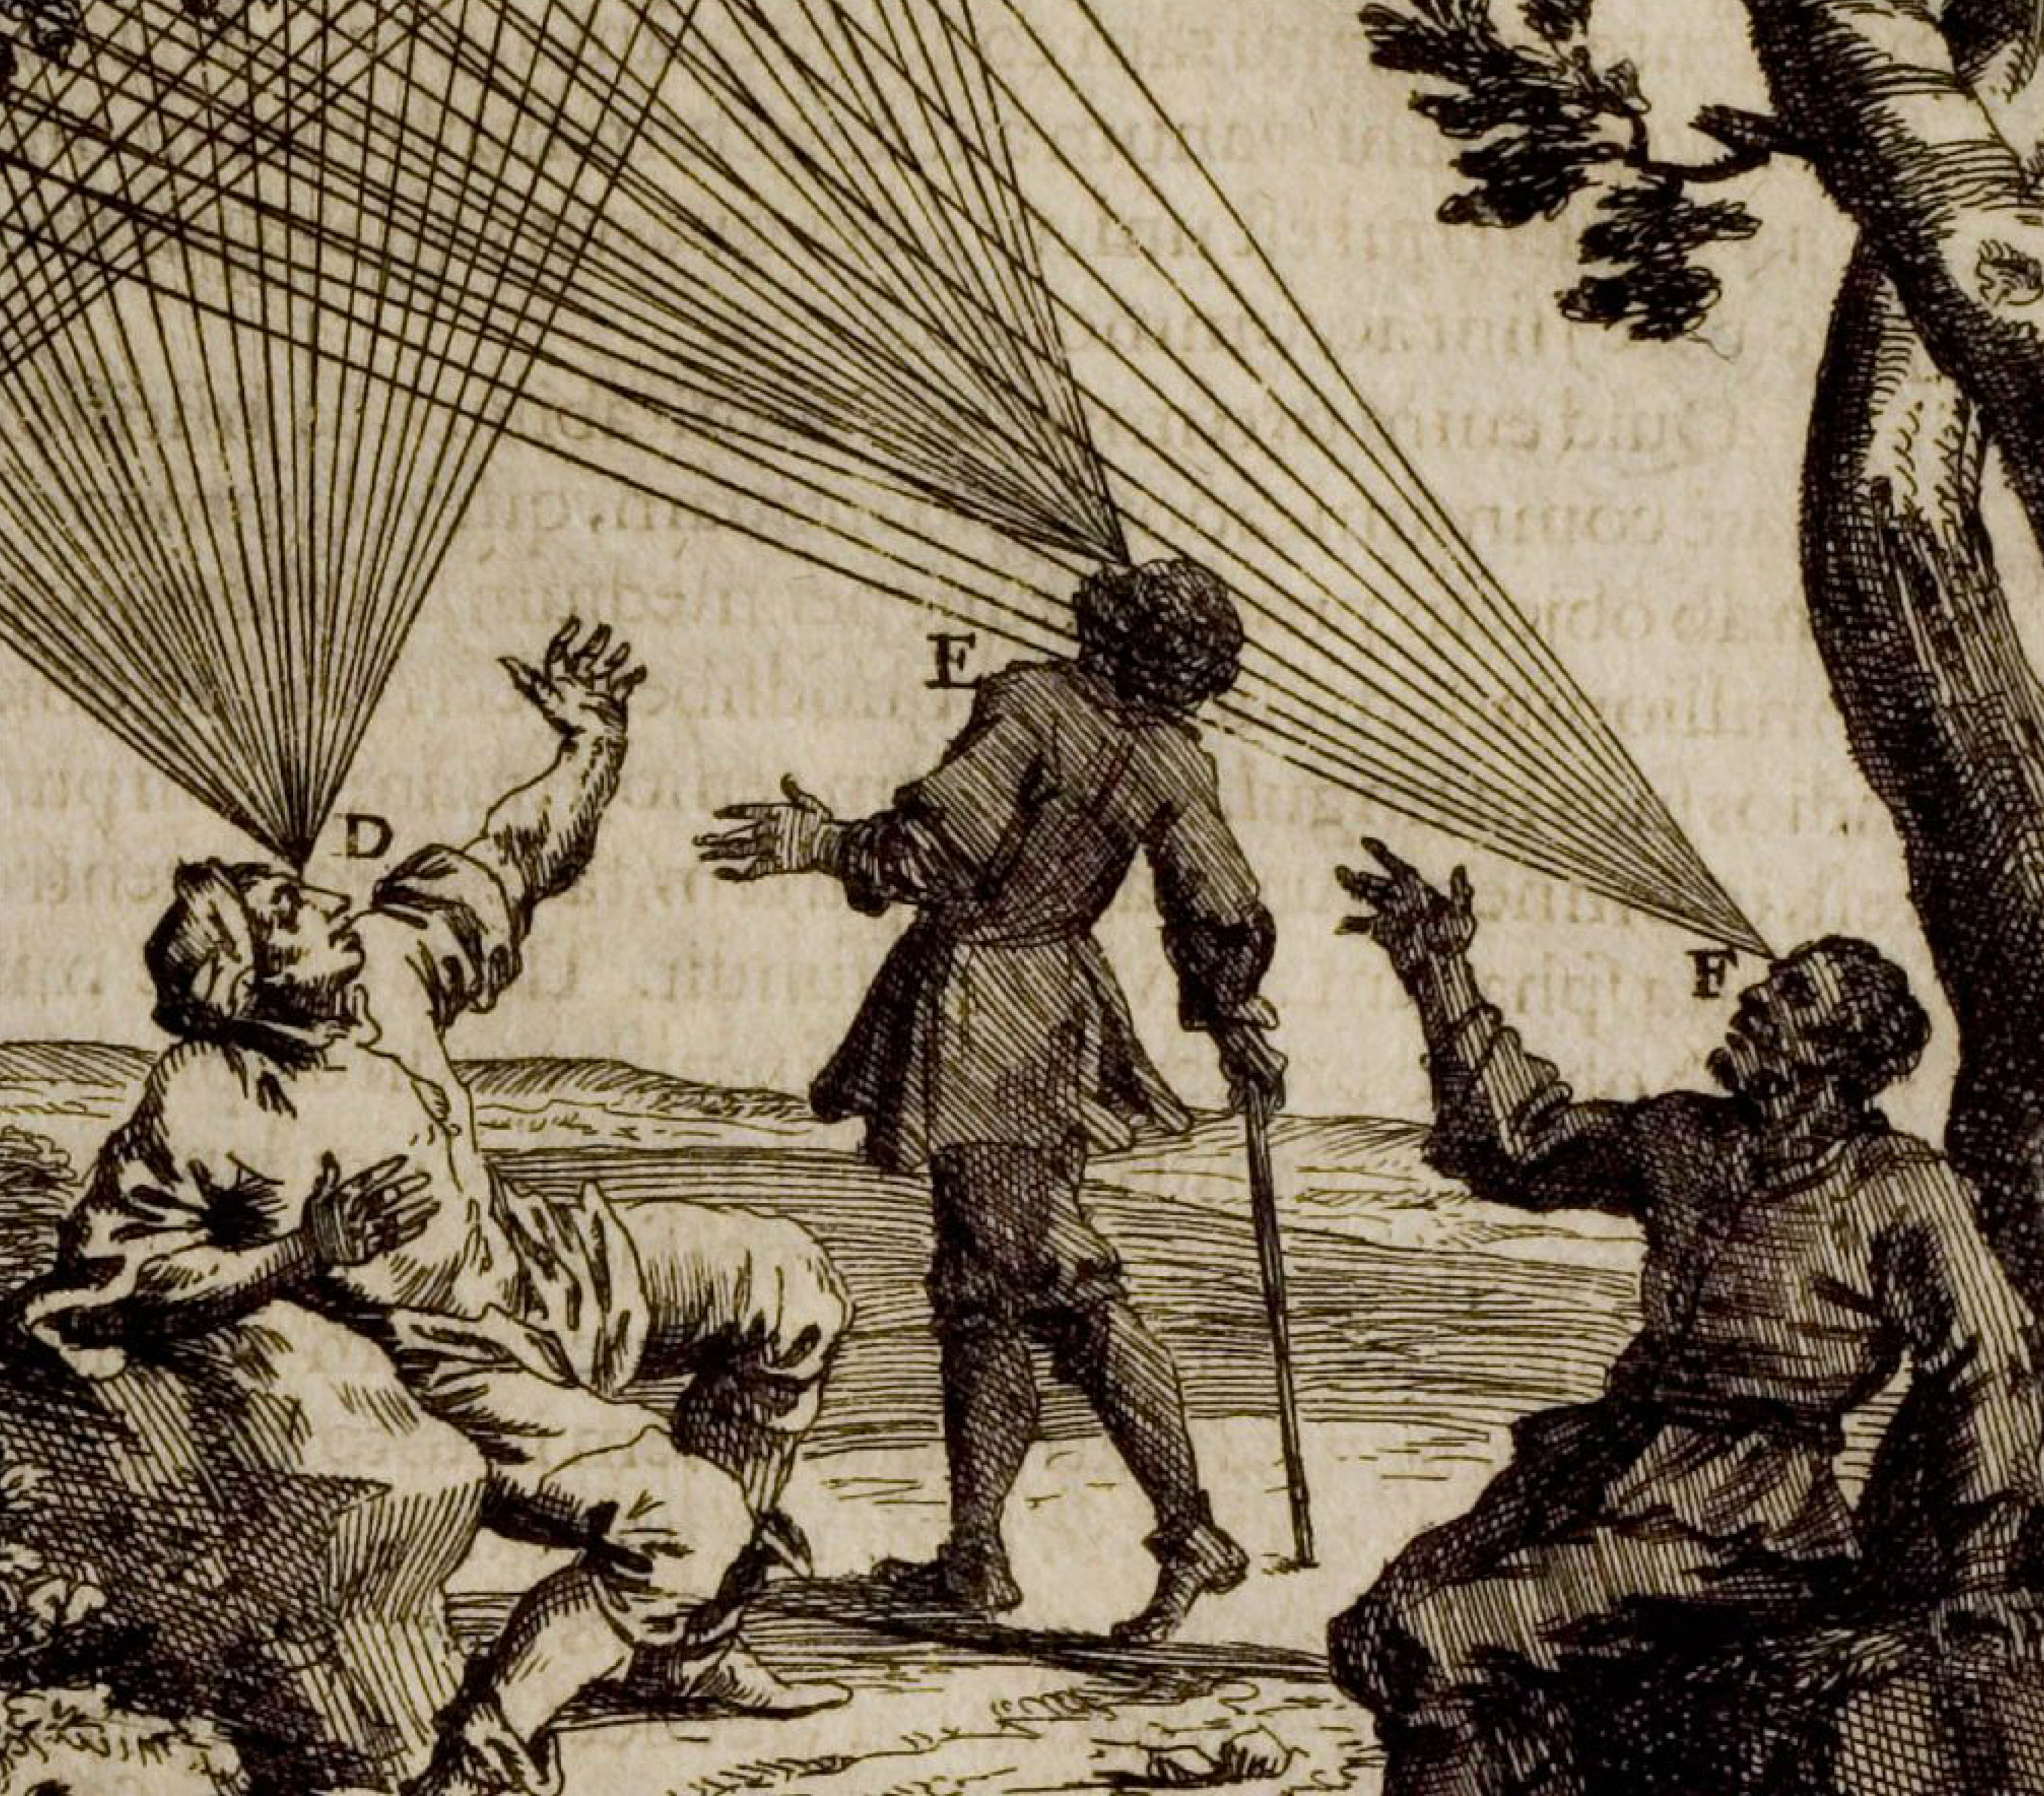
\includegraphics[width=0.8\linewidth]{1}
		\caption{\small\textit{\color{duongvaotoanhoc}Barry Mazur. Ảnh: Lance Murphey.}}
		\vspace*{-10pt}
	\end{figure}
	``Tôi bị cuốn hút bởi cách mà `hành động từ xa' này có thể xảy ra, và hoài nghi mọi giải thích về điều đó", ông nói. ``Tôi tự cho mình là `một triết gia về điện tử', và đăng ký vào Viện Công nghệ Massachussetts (MIT) với hy vọng theo đuổi một con đường với những mô tả nghề nghiệp như vậy. Nhưng ngay khi đặt chân đến đó, tôi phát hiện ra rằng những gì mà tôi từng nghĩ là `triết học về điện tử', thì mọi người gọi là toán học."
	\vskip 0.05cm
	Ngay khi bắt đầu học toán một cách nghiêm túc, Mazur trở nên quan tâm đến các vật thể rối rắm  hơn rất nhiều so với những loại sóng vật lý mang đến cho chúng ta âm thanh: các nút. Như chúng ta đã biết từ những trải nghiệm đau đớn của bản thân, các nút thắt hay đánh lừa mắt ta, chúng thay đổi hình dạng ngay trước mắt ta khi chúng ta cố gắng gỡ rối chúng. Chúng là những đối tượng nghiên cứu hoàn hảo của các nhà toán học, không hẳn vì điều đó có thể giúp chúng ta gỡ rối các nút thắt trong cuộc sống thực, mà vì sự hồi hộp và phấn khích mà việc nghiên cứu chúng đem lại. ``Lý thuyết nút thật tuyệt vời, nếu quan tâm đến nó, bạn sẽ có cảm giác rằng trực giác hình học của bạn ngày càng mở rộng," Mazur nói.
	\vskip 0.05cm
	Điều đầu tiên bạn nhận ra khi nhìn vào các nút là hình dạng và kích thước chính xác của chúng không phải là điều quan trọng. Điều đặc trưng cho một nút liên quan đến cách nó bị làm rối, chứ không phải là cách nó được đặt trong không gian như thế nào. Hình học cổ điển, với các khái niệm chính xác về hình dạng và kích thước, không quá hữu ích ở đây. Thay vào đó, những gì bạn cần là những khái niệm uyển chuyển hơn trong tô pô. Lĩnh vực toán học này coi hai hình dạng là giống nhau nếu một hình có thể bị biến dạng thành hình kia bằng cách kéo căng, ép hoặc uốn cong, nhưng không làm những hành động mạnh bạo hơn như cắt hình hoặc dán các mảnh của nó lại với nhau. Tô pô đôi khi được gọi là \textit{hình học của miếng cao su}.
	\vskip 0.05cm
	\textbf{\color{duongvaotoanhoc}Không nút}
	\vskip 0.05cm
	Mazur theo học tiến sĩ với tư duy tô pô đó. Công việc liên quan đến thứ mà  bạn có thể nghĩ là loại nút đơn giản nhất: một chiếc vòng đơn, hình dạng mà bạn có được từ một vòng dây chun không bị xoắn. Bạn có thể đặt một cái vòng như vậy lên mặt bàn theo vô số cách mà không phá vỡ cấu trúc trơn tru không bị thắt nút của nó. Và vì bản thân chiếc vòng là một vòng tròn bị biến dạng, miền bên trong và miền bên ngoài của vòng dây trên bàn chỉ đơn thuần là các phiên bản biến dạng của miền bên trong và miền bên ngoài của một đường tròn -- thực tế trực quan này được phát biểu một cách chính xác về mặt toán học bởi \textit{định lý đường cong Jordan}.
	\vskip 0.05cm
	Công trình tiến sĩ của Mazur thực hiện điều mà các nhà toán học thường làm khi họ có một kết quả nào đó về hình học hoặc tô pô: họ hỏi liệu nó có còn đúng hay không trong các không gian có số chiều cao hơn. Lý do họ làm được điều này là vì họ có thể -- họ có cách mô tả những hình dạng có số chiều cao hơn mặc dù chúng ta không thể hình dung được. Những hiểu biết sâu sắc về toán học thường nằm ẩn trong những không gian chiều cao hơn đó.
	\begin{figure}[H]
		\centering
		\vspace*{-5pt}
		\captionsetup{labelformat= empty, justification=centering}
		\includegraphics[width=0.85\linewidth]{2}
		\caption{\small\textit{\color{duongvaotoanhoc}Hình vẽ  mô tả cái gọi là không nút  (trên cùng bên trái) cũng như các nút nguyên tố khác được xác định bằng số lần tự thắt. Các nút nguyên tố, theo một nghĩa nào đó, chính là các nút không thể phân tích được.}}
		\vspace*{-10pt}
	\end{figure}
	Trong luận án tiến sĩ của mình, Mazur đã chứng minh một phiên bản nhiều chiều của định lý đường cong Jordan, đúng cho số chiều bất kỳ. Nó thường được gọi là \textit{Bài toán Schoenflies}. (Trong không gian ba chiều, chúng ta vẫn có thể hình dung được bài toán này: nó hỏi rằng những mặt cầu bị biến dạng có thể được đặt trong không gian ba chiều như thế nào.)
	\vskip 0.05cm
	Công trình của Mazur đã làm nảy sinh ra một trong nhiều khái niệm toán học  mang tên ông: \textit{ngụy biện Mazur}. Nó được gọi như vậy vì liên quan đến một lập luận toán học thông minh mà lẽ ra thực sự không nên được cho phép, nhưng, trong ngữ cảnh mà Mazur đang xem xét, hóa ra lại hoàn toàn hợp lệ. Bạn đọc hãy tìm tới phần phục lục để nắm được ý chính của ngụy biện Mazur.
	\vskip 0.05cm
	Mặc dù thực sự là một kết quả trong tô pô, nhưng định lý đường cong Jordan gợi ý về một cách tiếp cận thường được áp dụng trong lý thuyết nút: thay vì nhìn vào chiếc nút, họ nhìn vào một không gian mà họ tưởng tượng chiếc nút sẽ nằm trong đó, trừ đi chính nút đó. Không gian phi nút này có thể cho bạn biết nhiều điều về chính chiếc nút. Mazur đã giúp phát triển những hiểu biết sâu sắc về toán học cần thiết để khám phá nó. Thật kỳ lạ, cách tiếp cận cũng đưa ông tới một lĩnh vực không liên quan gì đến nút: lý thuyết số.
	\vskip 0.05cm
	\textbf{\color{duongvaotoanhoc}Từ những chiếc nút đến những con số} 
	\vskip 0.05cm
	Đơn giản một cách bất ngờ, lý thuyết số quan tâm đến các số nguyên $1$, $2$, $3$, $4$, v.v. và số học của chúng. Ví dụ, một nhà lý thuyết số có thể hỏi: liệu có ba số nguyên $a, b$ và $c$, thỏa mãn phương trình sau hay không:
	\setlength{\abovedisplayskip}{5pt}
	\setlength{\belowdisplayskip}{5pt}
	\begin{align*}
		a ^ 2 + b ^ 2 = c ^ 2. 
	\end{align*}
	Trong ví dụ này, câu trả lời là có. Ví dụ: $ a = 3 $, $ b = 4 $ và $ c = 5 $ thỏa mãn vì 
	\begin{align*}
		3 ^ 2 + 4 ^ 2 = 9 + 16 = 25 = 5 ^ 2.
	\end{align*}
	Các số nguyên tố có vai trò đặc biệt quan trọng trong lý thuyết số. Chúng là những số chỉ chia hết cho $1$ và chính bản thân chúng, chẳng hạn như $2$, $3$, $5$, $7$ và $11$. Bởi vì chúng không thể được phân tích thành tích của các số nhỏ hơn, chúng thường được coi là những nguyên tử của lý thuyết số: nếu bạn muốn chứng minh điều gì đó đúng với tất cả các số nguyên, việc chứng minh điều đó đúng với các số nguyên tố thường đã được coi là hoàn thành một chặng đường dài, vì việc chỉ ra điều đó đúng cho các số khác thường sẽ dễ dàng hơn.
	\vskip 0.05cm
	Số ít các số nguyên tố đầu tiên tập trung khá gần nhau, nhưng khi các số nguyên tố  tăng dần lên, chúng trở nên thưa thớt hơn. Chúng ta biết rằng có vô số số nguyên tố, nhưng cách chúng được phân bố giữa các số khác vẫn còn là một điều bí ẩn. Đó là chủ đề của một trong những bài toán mở lớn nhất trong toán học, được gọi là \textit{Giả thuyết Riemann}.
	\begin{figure}[H]
		\centering
		\vspace*{-5pt}
		\captionsetup{labelformat= empty, justification=centering}
		\includegraphics[width=0.9\linewidth]{3}
		\caption{\small\textit{\color{duongvaotoanhoc}Nhà toán học Hy Lạp cổ đại Euclid đã chứng minh rằng có vô hạn số nguyên tố. Ông là người cầm chiếc com--pa trong bức tranh Trường phái Athens của Raffaello Sanzio.}}
		\vspace*{-10pt}
	\end{figure}
	Lý thuyết số nổi tiếng với việc đặt ra những bài toán tưởng chừng dễ dàng nhưng hóa ra lại cực kỳ khó chứng minh. Trong một bài báo thú vị viết vào năm $1991$, Mazur đã so sánh những bài toán đó với những bông hoa đẹp đẽ và đầy cám dỗ, ông viết rằng, ``lý thuyết số chứa bầy bọ luôn chực chờ cắn những người yêu hoa bị cám dỗ, những người sau khi bị cắn được truyền cảm hứng để nỗ lực hết sức mình".
	\vskip 0.05cm
	Tuy nhiên, bông hoa đã cám dỗ Mazur không phải là một phương trình đơn giản hay một câu nói dễ hiểu -- ông đã phát hiện ra hình ảnh ví von đó rằng nếu bạn coi các số nguyên tố tương tự như những chiếc nút và các số nguyên khác tương tự như một không gian bao quanh nút, thì bạn có thể điều chỉnh những ý tưởng mạnh mẽ của lý thuyết nút để áp dụng vào lý thuyết số. Theo ông: ``Ý tưởng chuyển đổi từ ngôn ngữ nút thành ngôn ngữ của các con số rất thú vị. Nó không chỉ rất thích thú mà còn là con đường tốt để có trực giác về các bài toán trong lý thuyết số."
	\vskip 0.05cm
	Một kết quả của phương pháp này là một chứng minh của \textit{Giả thuyết chính Iwasawa}, mà Mazur đã tìm ra cùng với Andrew Wiles vào đầu những năm $1980$. Chứng minh đó có thể được xem như một phiên bản tương tự của giả thuyết Riemann trong một bối cảnh khác so với giả thuyết được đề cập ở trên. Nó cũng dẫn Mazur đến những kết quả quan trọng khác, và quan trọng hơn cả, đã đặt ra những hướng đi mới trong lý thuyết số.
	\vskip 0.05cm
	\textbf{\color{duongvaotoanhoc}Một bông hoa nổi tiếng}
	\vskip 0.05cm
	Việc chứng minh, hoặc thậm chí chỉ là phát biểu, giả thuyết chính Iwasawa đòi hỏi những kiến thức toán học chuyên sâu mà chúng ta không thể trình bày ở đây. Tuy nhiên, những gì chúng ta có thể làm là đến thăm một trong những bông hoa đầy cám dỗ đã thôi thúc nhiều thế hệ nhà toán học nỗ lực hết sức. Trong ví dụ đã đưa ra ở trên, chúng ta tìm thấy một bộ ba số nguyên thỏa mãn phương trình
	\begin{align*}
		a ^ 2 + b ^ 2 = c ^ 2.
	\end{align*}
	Trên thực tế, có vô số bộ như vậy, được gọi là những \textit{bộ ba Pythagore}.
	\vskip 0.05cm
	Nhưng điều gì sẽ xảy ra nếu chúng ta thay thế số mũ $ 2 $ trong phương trình bằng $ 3 $: 
	\begin{align*}
		a ^ 3 + b ^ 3 = c ^ 3.
	\end{align*}
	Khi đó phương trình nhận được có nghiệm nguyên không? Điều gì sẽ xảy ra nếu chúng ta thay thế số mũ bằng $ 4, 5, 6, $ hoặc bất kỳ số nguyên dương $ n $ nào khác? Năm $1637$, nhà toán học người Pháp Pierre de Fermat đã tìm ra câu trả lời là ``không". Khi số mũ trong phương trình là một số nguyên lớn hơn $ 2 $ thì không có nghiệm nguyên nào mà cả ba số đều khác $ 0 $. Fermat viết nguệch ngoạc bên lề một cuốn sách rằng ông đã tìm thấy một ``chứng minh tuyệt vời" cho điều này, nhưng lề quá nhỏ để có thể viết được chứng minh.
	\vskip 0.01cm
	Chính những nét chữ nguệch ngoạc này đã đặt các nhà toán học vào một nỗ lực kéo dài ba thế kỷ để tìm ra chứng minh cho cái được gọi là \textit{Định lý cuối cùng của Fermat}.
	\vskip 0.01cm
	Như bạn có thể hình dung được, hành trình tìm ra chứng minh đó đã đưa các nhà toán học đến những hiểu biết sâu rộng về toán học mà nếu nhìn bề ngoài, bạn sẽ không ngờ có liên quan đến bài toán này. Một điều trở nên rõ ràng vào những năm $1970$ là một lớp phương trình khác sẽ đóng vai trò quan trọng trong việc nghiên cứu Định lý cuối cùng của Fermat. Chúng được gọi là các \textit{đường cong elliptic}, cho bởi các phương trình có dạng
	\begin{align*}
		y ^ 2 = x ^ 3 + ax + b,
	\end{align*}
	trong đó $ a $ và $ b $ là các số nguyên.
	\vskip 0.01cm
	Như bạn có thể nhớ lại những kiến thức toán học đã học ở trường phổ thông, khi học về các hình như đường tròn hoặc parabol, thì một phương trình cũng có thể xác định một đường cong. Thật ngạc nhiên, hình dạng của những đường cong như vậy có thể cho bạn biết rất nhiều về các nghiệm của  các phương trình liên quan và do đó cực kỳ thú vị đối với các nhà lý thuyết số.
	\vskip 0.01cm
	Mazur là một trong những nhà toán học đã dồn nhiều nỗ lực vào nghiên cứu các đường cong elliptic, và trên thực tế, chúng đóng một vai trò quan trọng trong \textit{Giả thuyết chính Iwasawa} đã nói đến ở trên. Bằng cách khai thác các tính chất đối xứng đẹp đẽ của các nghiệm nằm trên các đường cong, Mazur thành công trong  việc chứng minh cái gọi là \textit{Giả thuyết xoắn} cho các đường cong elliptic. Kết quả này, ngoài việc bản thân nó là một kết quả ``vô cùng đẹp và thanh thoát", theo lời dẫn của Giải thưởng Chern, còn khởi xướng những lĩnh vực nghiên cứu mới, mở đường cho chứng minh định lý cuối cùng của Fermat. Điều này cuối cùng đã được hoàn thành vào năm $1994$, hơn $350$ năm sau nét bút nguệch ngoạc của Fermat, bởi Andrew Wiles, một cộng sự của Mazur.
	\vskip 0.05cm
	\textbf{\color{duongvaotoanhoc}Toán học là cá nhân}
	\vskip 0.05cm
	Huy chương Chern được trao cho những thành tựu trọn đời trong toán học. Những gì chúng ta đã đề cập trong bài viết này chỉ là một phần nhỏ trong nghiên cứu của Mazur.
	\vskip 0.05cm
	Lời giới thiệu của giải thưởng về ông mô tả ông là người có ``quan điểm đa nguyên" về toán học. ``Mỗi người đều có một  cách nào đó để tiếp cận thế giới bằng những cảm nhận, trực giác và trải nghiệm toán học hoặc gần với toán học," ông đã trả lời như vậy khi chúng tôi hỏi ông nghĩ điều đó có nghĩa là gì. ``Và những cách tiếp cận và thiên hướng toán học này, sau cùng, mang tính cá nhân và không thể được phân loại bằng cách dán nhãn thô thiển."
	\vskip 0.05cm
	Mazur cũng được vinh danh vì công lao dẫn dắt và sự bao dung mà ông dành cho những người mới bắt đầu sự nghiệp, bao gồm gần $60$ nghiên cứu sinh tiến sĩ mà ông đã hướng dẫn. Khi chúng tôi hỏi điều gì khiến ông thấy thích khi làm việc với thế hệ tiếp theo, câu trả lời của ông ấy rất đơn giản: ``Hầu hết thời gian  họ dạy tôi nhiều hơn là tôi dạy họ."
	\vskip 0.05cm
	\textbf{\color{duongvaotoanhoc}Phụ lục: Ngụy biện của Mazur}
	\vskip 0.05cm
	Trước tiên, chúng ta hãy xem xét tổng vô hạn sau:
	\begin{align*}
		S = 1-1 + 1-1 + 1-1 + 1-1\ldots
	\end{align*}
	Nó được gọi là chuỗi Grandi, theo tên nhà toán học, triết học và linh mục người Ý Guido Grandi ($1671-1742$).
	\vskip 0.05cm
	Nếu chúng ta nhóm các số hạng của nó theo cách sau đây: 
	\begin{align*}
		S \!=\! (1\!-\!1) \!+\! (1\!-\!1) \!+\! (1\!-\!1) \!+\! (1\!-\!1) \!+\! \ldots
	\end{align*}
	thì chúng ta có thể tin rằng giá trị của $S$ phải bằng $0$ bởi vì biểu thức trong mỗi dấu ngoặc đơn đều bằng $0$. Tuy nhiên, không có gì ngăn cản chúng ta nhóm các số hạng của nó theo một cách khác, chẳng hạn
	\vskip 0.15cm
	\centerline{$S \!=\! 1 \!+\! (\!-\! 1 \!+\! 1) \!+\! (\!-\! 1 \!+\! 1) \!+\! (\!-\! 1 \!+\! 1) \!+\! \ldots$}
	\vskip 0.05cm
	Cách nhóm các số hạng này dẫn đến niềm tin rằng giá trị của $S$ phải bằng $1$, vì biểu thức trong mỗi dấu ngoặc đứng sau số $1$ đầu tiên đều bằng $0$.
	\vskip 0.05cm
	Điều đó cho thấy rằng $S$ bằng cả $0$ và $1$, nói cách khác, $0 = 1$! Vì điều này không đúng nên có gì đó sai trong lập luận của chúng ta. Vấn đề nằm ở chỗ các tổng vô hạn không thể được xử lý theo cách giống như các tổng hữu hạn.
	\vskip 0.05cm
	Tuy nhiên, có những bối cảnh mà ở  đó một lập luận tương tự như ở trên trở nên đúng đắn. Sau đây chính là cách Mazur giải thích ngụy biện của ông.
	\vskip 0.05cm
	Giả sử bạn có (mà bạn nghĩ là vô số cái khác nhau) những đối tượng toán học được gắn nhãn bằng các số
	\begin{align*}
		[- \infty], .., [-2], [-1], [0], [+1], [+2], ..., [+\infty]
	\end{align*}
	(Đúng thế: $[\pm {\infty}] $)
	\vskip 0.05cm
	Hơn nữa, giả sử rằng bạn có thể ghép chúng lại với nhau như những toa tàu, sau đó cộng các số trong nhãn của chúng với nhau, và giả sử rằng đối tượng được tạo thành cũng là một đối tượng trong bộ sưu tập của bạn và có nhãn tương ứng với tổng các nhãn nhận được. Ví dụ: $ [1] + [1] = [2]$. 
	\vskip 0.05cm
	Ngoài ra, giả sử bạn thậm chí có thể ghép  được những đoàn tàu dài vô tận, ví dụ:
	\begin{align*}
		[0] = [0] + [0] + [0] + [0] + \ldots
	\end{align*}
	Khi đó, nếu loại thao tác chúng ta đã thực hiện đối với tổng $S$ ở trên là hợp lệ trong ngữ cảnh mà chúng ta đang xem xét, thì chúng ta có thể chứng minh rằng
	\begin{align*}
		[0] = [ 1].
	\end{align*}
	Điều đó cũng có nghĩa
	\begin{align*}
		 [2] &= [1] + [1] = [0] + [0] = [0],\\
		[3] &= [1] + [1] + [1] = [0] + [0] + [0] = [0],
	\end{align*}
	và những đẳng thức tương tự như thế.
	\vskip 0.05cm
	Điều này dẫn tới rằng tất cả các đối tượng chúng ta quan tâm thực ra là một. Không có vô số đối tượng, mà chỉ có một!
\end{multicols}